\documentclass[jair,twoside,11pt,theapa]{article}
\usepackage{jair, theapa, rawfonts}
\usepackage{graphicx}  % include figures
\usepackage{amsmath}  % for centering equations

\jairheading{?}{YYYY}{1-??}{M/YY}{M/YY}
\ShortHeadings{Standard Machine Learning Language (SML)}
{Ikegwu, Hao, \& Brunner}
\firstpageno{1}

\begin{document}

\title{Standard Machine Learning Language}

\author{\name Kelechi Ikegwu \email ikegwu2@illinois.edu \\
       \addr 226 Astronomy Building, MC-??? \\1002 W. Green St.\\ Urbana, IL  61801
       \AND
       \name Micheal Hao  \email ???@illinois.edu \\
       \addr ???
       \AND
       \name Robert Brunner \email bigdog@illinois.edu\\
       \addr 226 Astronomy Building, MC-221 \\1002 W. Green St.\\ Urbana, IL  61801}

% For research notes, remove the comment character in the line below.
% \researchnote

\maketitle


\begin{abstract}
Standard Machine Learning Language (SML) is a language agnostic framework that integrates a query-like language to simplify the development for a variety of state-of-the-art machine learning pipelines. Emphasis was placed on ease of use and abstracting the complexities of machine learning from the end user encouraging it's use in professional and academic settings from a variety of disciplines. SML's architecture is discussed, followed by multiple interfaces that one could use to interact with SML. We then apply SML to a few research problems and compare the complexities for multiple problems. Lastly we perform a case study on SML. The source code and documentation for SML is open sourced and publicly available on github \cite{ginsberg}.
\end{abstract}

\section{Introduction}
\label{Introduction}

Machine Learning has simplified the process of solving a vast amount problems in a variety of fields by learning from data. In most cases machine learning has become more attractive than manually creating programs to solve these same issues. However they're a lot of nuisances (that a novice may be unfamilar with) involved when developing machine learning pipelines \cite{pedros:fewUsefulThings} and if they are not taken into consideration one may not receive satisfactory results. In addition to this, an experience user may not want to deal with [REASONS HERE]. In this paper we introduce Standard Machine Learning Language (SML)  which helps to combat these two use cases.


The overall objective of the SML is to provide a level of abstraction which simplifies the development process of machine learning pipelines. Consequently this enables researchers and industry professionals without a background in this area to use machine learning to solve problems. We developed a query like language to which serves as an abstraction from writing actual machine learning code see Figure \ref{fig:sml-ex-1} for an example.   

\begin{figure}
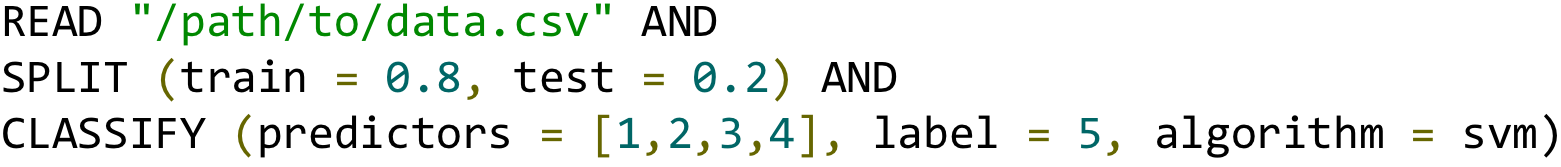
\includegraphics[width=0.6\textwidth]{figs/sml-ex-1.png}
\centering
\caption{Example of a SML Query. TODO: FIX COLOR SYNTAX}
\label{fig:sml-ex-1}
\end{figure}

\section{Related Works}
\label{RelatedWorks}

TPOT \cite{TPOT} is a tool implemented in python that creates and optimizies machine learning pipelines. Given cleaned data, TPOT performs feature selection, preprocessing , and construction. Given the task (classification, regression, or clustering) it uses the best features to determine the most optimal model to use. Lastly, it performs optimization on parameters for the selected model. What differentiates TPOT from SML is that in addition feature, model, and parameter selction/optimization a framework is explictly in place to apply these models to different datasets and construct visualizations for different metrics with each algorithm.

\section{Grammar}
\label{grammar}

The SML language is a domain specific language with grammar implemented in Bakus-Naur form (BNF) \cite{BNF}. Each expression has a rule and can be expanded into other terms. Figure \ref{fig:sml-ex-1} is a typical example of how one would perform classifcation on a dataset. The query in Figure \ref{fig:sml-ex-1} reads in a dataset, peforms a split 80/20 split of training and testing data respectively, and performs classifcation of the 5th column of the hypothetical dataset using columns 1-4 as predictors. 

\subsection{Grammar Structure}
In this subsection we define the grammar of SML in terms of BNF. A query can be defined by a delimited list of actions where the delimiter is an "AND" statement; with BNF syntax this is defined as:
\begin{equation} \label{BNF:Query}
<Query> ::= <Action> | <Action> “AND” <Query>
\end{equation}

An action in (\ref{BNF:Query}) follows one of the following structures defined in (\ref{BNF:Action}) where a keyword is required followed by an argument and/or option list.
\begin{equation} \label{BNF:Action}
\begin{split}
<Action> ::= <Keyword> “<Argument>” \\
| <Keyword> “<Argument>” “(”<Option List>“)” \\
| <Keyword> “(”<Option List>“)”
\end{split}
\end{equation}

A keyword is a predefined term associating an Action with a particular string. An Argument generally is a single string surrounded by quotes that specifies a path to a file. Lastly, an Arugment can have a multitude of options (\ref{BNF:Option}) where an Option consist of an OptionName with either an option value or option value list. An OptionName, and OptionValue consist of a single string, an OptionList (\ref{BNF:OptionList}) consist of a comma delimited list of options and an OptionValueList (\ref{BNF:OptionValueList}) consist of a comma delimited list of OptionValues.

\begin{equation} \label{BNF:Option}
\begin{split}
<Option> ::= <Option Name> “=” <Option Value> \\
		| <Option Name> “=” “[”<Option Value List>“]”
\end{split}
\end{equation}

\begin{equation} \label{BNF:OptionList}
\begin{split}
	<Option List> ::= <Option> | <Option> “,” <Option List>
\end{split}
\end{equation}

\begin{equation} \label{BNF:OptionValueList}
\begin{split}
<Option Value List> ::= <Option Value> \\
| <Option Value> “,” <Option Value List>
\end{split}
\end{equation}

Figure \ref{SML:BNFComp} % figure that shows Figure 1 and it in BNF format side by side.

\subsection{Keywords}
In this subsection we define all of the available keywords that exist in SML. Currently they're 8 keywords

\subsubsection{Reading Datasets}
When reading data from SML one must use the \(READ\) keyword followed by an Argument containg a path to the dataset. Figure \ref{SML:READ} shows examples of the \(READ\) keyword being used. \(READ\) also accepts an OptionList, for a full list of the optional arguments can visit \ref{}.

\subsubsection{Cleaning Data}
When NaNs, NAs and/or other troublesome values are present in dataset we clean these values in SML by using the \(REPLACE\) keyword. Figure \ref{SML:REPLACE} shows can exajmple of the \(REPLACE\) keyword being used.  

\subsubsection{Patitioning Datasets}
For majority of the situations in Machine Learning it's often useful to split a dataset into training and testing datasets. This can be achieved in SML by using the \(SPLIT\) keyword. Figure \ref{SML:SPLIT} show an example utlizing the \(SPLIT\) keyword.

\subsubsection{Using Classification Algorithms}


\subsubsection{Using Clustering Algorithms}

\subsubsection{Using Regression Algorithms}

\subsubsection{Saving/Loading Models}

\subsubsection{Visualizating Datasets and Metrics of Algorithms}

\section{SML's Architecture}
\label{sml-architecture}

Architecture Stuff

\subsubsection{Model Phase}
model phase
\subsubsection{Apply Phase}
apply phase
\subsubsection{Metrics Phase}
It's often useful to visualize the data that one works with; it's also beneifical to see the performance metrics of your machine learning algorithm to better understand ones data. By default if you specify the `PLOT` keyword in a query, SML will execute the metrics phase. Figure \ref{fig:metric-phase} displays a block diagram of the metric phase of SML. SML performs a dictionary lookup with the average complexity of O(1) to find specific terms that are in the query. For the example in Figure \ref{fig:metric-phase} we specified `PLOT` which instructs SML to create visualizations, with the `READ` keyword SML will create a lattice plot containing Kernel Density Estimates. Given an algorithm type such as Classification SML generates plots such as ROC Curves and Validation and Learning Curves. For a comprehensive list for the type of plots that SML can generate visit  \cite{}.

\begin{figure}
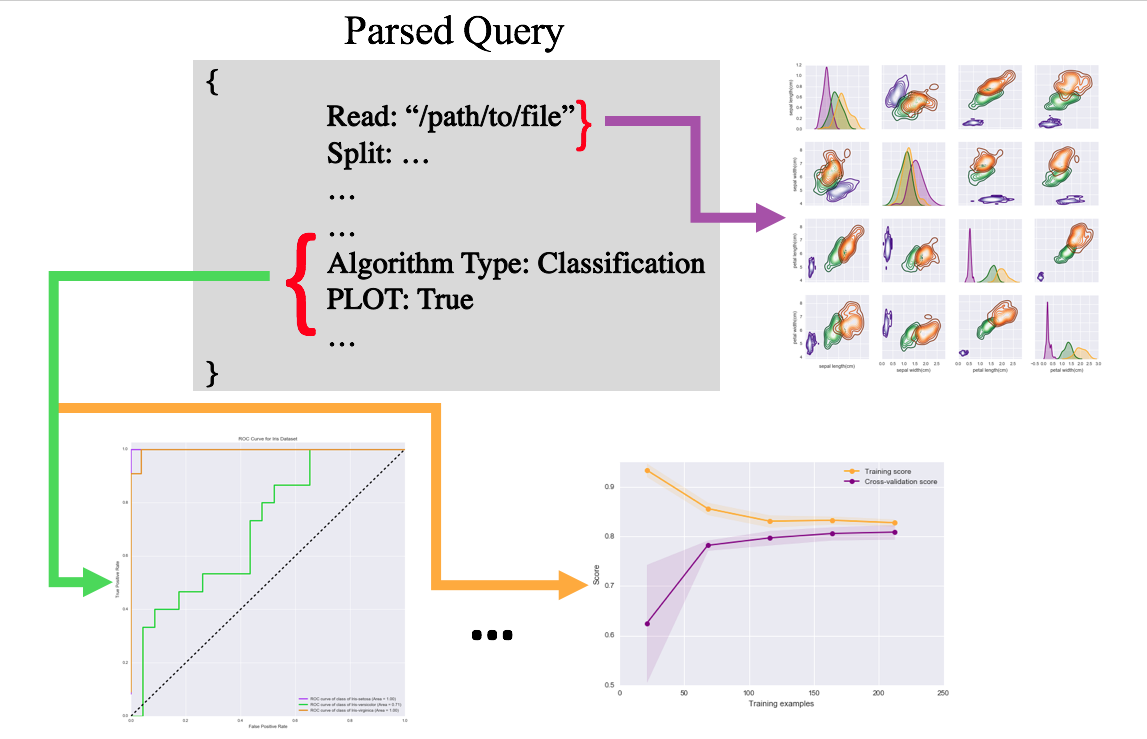
\includegraphics[width=0.6\textwidth]{figs/metric-phase.png}
\centering
\caption{Block Diagram of Metric Phase Architecture}
\label{fig:metric-phase}
\end{figure}

\subsubsection{Parser}
parser

\subsubsection{Connector}
connector

\section{Interface}
\label{interface}

They're multiple interfaces available for working with SML. We've developed a web tool that's publicly available which allows the user to interact with SML. There's also a REPL environment available that allows the user to interactively use SML. Lastly, users have the option to import SML into an existing pipeline to simplify the development process.

\section{Use Cases}
\label{use-cases}

use case stuff

\section{Case Study}
\label{case-study}
case study stuff

\section{Future Work}
\label{future-work}

future work stuff

\section{Conclusion}
\label{conclusion}
conclusion stuff

\acks{acknowledgments go here}

\appendix
\section*{Appendix X...}

Appendix goes here if needed.

\vskip 0.2in
\bibliography{main}
\bibliographystyle{theapa}

\end{document}






